\documentclass[11pt]{article}
\usepackage{a4wide}
\usepackage{amsmath}
\usepackage{amssymb}
\usepackage{amsthm}
\usepackage{cite}
\usepackage{subfig}
\usepackage{graphicx}
\usepackage{hyperref}
\usepackage{color}
\usepackage{xspace}
\usepackage[ruled, noline, algo2e, noend, linesnumbered]{algorithm2e}

\newcommand{\todo}[1]{\xspace{\bfseries\sffamily\textcolor{red}{[#1]}}\xspace}

\newtheorem{problem}{Problem}[section]
\newtheorem{definition}{Definition}[section]
\newtheorem{theorem}{Theorem}[section]
\newtheorem{lemma}[theorem]{Lemma}
\newtheorem{proposition}[theorem]{Proposition}
\newtheorem{corollary}[theorem]{Corollary}

\author{M.~El-Kebir, G.W.~Klau}
\title{Fragment-based molecule parameterisation}

\begin{document}

\maketitle

\section{Introduction}

The automated topology builder (ATB) is a web server for generating topologies
of novel molecules compatible with the GROMOS 53A6 force field \cite{Malde11}.
The ATB is able to parameterise molecules consisting of up to 50 atoms. Due to
the complexity of the quantum mechanics computations, molecules larger than 50
atoms pose a problem for the ATB. 

Here, we introduce a method that assists the ATB by searching for fragments
common to both the input molecule and a molecule in the repository. The atom
charges of the input molecule are set according to the charges of the core atoms
of the found common fragments.

\section{Problem definition}

A molecule is a simple graph $G=(V,E)$ whose nodes and edges correspond to atoms
and bonds, respectively. Nodes are labeled by their partial charge $w : V
\rightarrow \mathbb{R}$ and their atom type $t : V \rightarrow \mathbb{N}$. 
For a subset $V^\prime \subseteq V$, $t(V^\prime)$ is the set $\bigcup_{v \in
V^\prime} t(v)$. The neighborhood $N(v)$ of a node $v \in V$ is the set $\{ u
\mid (u,v) \in E \}$. Similarly for a subset $V^\prime \subseteq V$, we define
$N(V^\prime)$ to be the set $\bigcup_{v \in V^\prime} N(v)$. 

Given molecules $G_1 = (V_1, E_1)$ and $G_2 = (V_2, E_2)$ with atom types $t_1 :
V_1 \rightarrow \mathbb{N}$ and $t_2 : V_2 \rightarrow \mathbb{N}$, we define a
common fragment and its shell as follows.

\begin{definition}
  A \emph{common fragment} is a pair $(V^\prime_1, V^\prime_2)$ with $V^\prime_1
  \subseteq V_1$ and $V^\prime_2 \subseteq V_2$ that admits a bijection $h :
  V^\prime_1 \cup N(V^\prime_1) \rightarrow V^\prime \cup N(V^\prime_2)$ such
  that
  \begin{enumerate}
    \item[(i)] $G_1[V^\prime_1]$ and $G_2[V^\prime_2]$ are connected,
    \item[(ii)] $(u,v)$ is an edge in $G_1[V^\prime_1 \cup N(V^\prime_1)]$ if and
      only if $(h(u),h(v))$ is an edge in $G_2[V^\prime_2 \cup N(V^\prime_2)]$,
    \item[(iii)] $t_1(v) = t_2(h(v))$ for all $v \in V^\prime_1 \cup
      N(V^\prime_1)$.
  \end{enumerate}
\end{definition}
\begin{definition}
  The \emph{shell} of a common fragment $(V^\prime_1, V^\prime_2)$ is given
  by $(N(V^\prime_1), N(V^\prime_2))$.
\end{definition}

\begin{definition}
A common fragment $(V^\prime_1,V^\prime_2)$ is \emph{maximal} if
there exists no common fragment $(V^{\prime\prime}_1,V^{\prime\prime}_2)$ such
that $V^\prime_1 \subseteq V^{\prime\prime}_1$ and $V^\prime_2 \subseteq
V^{\prime\prime}_2$.
\end{definition}

The problem that we want to solve is now as follows. See
Figure~\ref{fig:example} for an example.

\begin{problem}
Given graphs $G_1 = (V_1, E_1)$ and $G_2 = (V_2, E_2)$ with atom types $t_1 :
V_1 \rightarrow \mathbb{N}$ and $t_2 : V_2 \rightarrow \mathbb{N}$, find the
set of all maximal common fragments.
\end{problem}

\todo{Extend $N(v)$ to variable shell size.}

\begin{figure}
  \center
  \subfloat[\label{fig:16481}$G_1$]{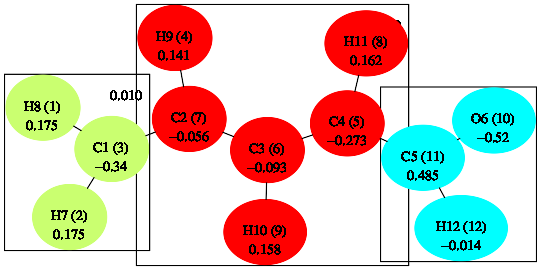
\includegraphics[width=.6\textwidth]{images/16841}}
  %\hspace{.5cm}
  \\
  \subfloat[$G_2$]{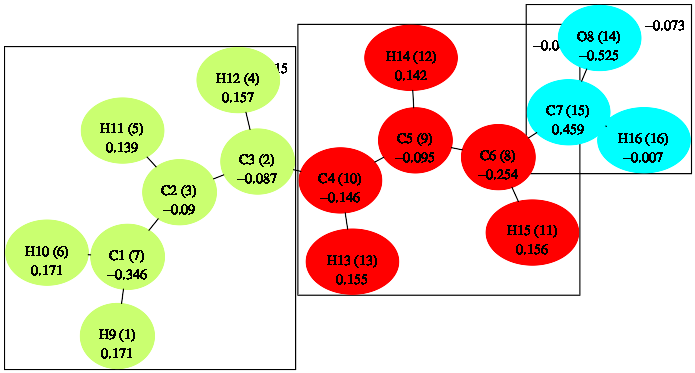
\includegraphics[width=.6\textwidth]{images/16842}}
  \\
  \subfloat[Maximal common fragments]{
    \centering
    \small
    \begin{tabular}{|lp{.8\textwidth}|}
      \hline
      1 & (C4~(5)~,~C5~(9)), (H11~(8)~,~H14~(12)), (C3~(6)~,~C6~(8)), (H10~(9)~,~H15~(11))\\
      2 & (C3~(6)~,~C6~(8)), (H10~(9)~,~H15~(11)), (C2~(7)~,~C5~(9)), (H9~(4)~,~H14~(12))\\
      3 & (C4~(5)~,~C3~(2)), (H11~(8)~,~H12~(4)), (C3~(6)~,~C2~(3)), (H10~(9)~,~H11~(5))\\
      4 & (C3~(6)~,~C2~(3)), (H10~(9)~,~H11~(5)), (C2~(7)~,~C3~(2)), (H9~(4)~,~H12~(4))\\
      5 & (C4~(5)~,~C3~(2)), (H11~(8)~,~H12~(4)), (C3~(6)~,~C4~(10)), (H10~(9)~,~H13~(13)), (C2~(7)~,~C5~(9)), (H9~(4)~,~H14~(12))\\
      6 & (C4~(5)~,~C4~(10)), (H11~(8)~,~H13~(13)), (C3~(6)~,~C5~(9)), (H10~(9)~,~H14~(12)), (C2~(7)~,~C6~(8)), (H9~(4)~,~H15~(11))\\
      7 & (C4~(5)~,~C2~(3)), (H11~(8)~,~H11~(5)), (C3~(6)~,~C3~(2)), (H10~(9)~,~H12~(4)), (C2~(7)~,~C4~(10)), (H9~(4)~,~H13~(13))\\
      8 & (C4~(5)~,~C5~(9)), (H11~(8)~,~H14~(12)), (C3~(6)~,~C4~(10)), (H10~(9)~,~H13~(13)), (C2~(7)~,~C3~(2)), (H9~(4)~,~H12~(4))\\
      9 & (C5~(11)~,~C7~(15)), (H12~(12)~,~H16~(16)), (O6~(10)~,~O8~(14)), (C4~(5)~,~C6~(8)), (H11~(8)~,~H15~(11)), (C3~(6)~,~C5~(9)), (H10~(9)~,~H14~(12)), (C2~(7)~,~C4~(10)), (H9~(4)~,~H13~(13))\\
      10 &(C1~(3)~,~C1~(7)), (H7~(2)~,~H10~(6)), (H8~(1)~,~H9~(1)), (C4~(5)~,~C4~(10)), (H11~(8)~,~H13~(13)), (C3~(6)~,~C3~(2)), (H10~(9)~,~H12~(4)), (C2~(7)~,~C2~(3)), (H9~(4)~,~H11~(5))\\
      \hline
    \end{tabular}
  }
  \caption{There are ten maximal common fragments.}
  \label{fig:example}
\end{figure}

\section{Method}

We solve the problem by finding maximal cliques on the node product graph, which
is defined as follows.

\begin{definition}
The \emph{node product graph} $G_1 \otimes G_2 = (V_{12}, E_{12})$ has node
set $V_{12} = \{(u,v) \in V_1 \times V_2 \mid t_1(u) = t_2(v), 
t_1(N(u)) = t_2(N(v)) \}$ and an edge in $E_{12}$ between $(u,v)$ and
$(u^\prime,v^\prime)$ if and only if $u \neq u^\prime$ and $v \neq v^\prime$,
and either $(u,u^\prime) \in E_1$ and $(v,v^\prime) \in E_2$, or $(u,u^\prime)
\not \in E_1$ and $(v,v^\prime) \not \in E_2$.
\end{definition}

Following \cite{Koch:2001wi}, we distinguish between $c$ and $d$-edges in the
product graph.

\begin{definition}
An edge $((u,v),(u^\prime,v^\prime)) \in E_{12}$ is a \emph{$c$-edge} if
$(u,u^\prime) \in E_1$ and $(v,v^\prime) \in E_2$, otherwise it is a
\emph{$d$-edge}.
\end{definition}

The $c$-neighborhood $N_c(v)$ of a node $v \in V_{12}$ is the set $\{ u
\mid (u,v) \in E_{12}, (u,v) \mbox{ is a $c$-edge} \}$. Conversely, $N_d(v)$ is
the $d$-neighborhood of a node $v \in V_{12}$.
%Similarly for a subset $V^\prime_{12} \subseteq V_{12}$, we define $N_c(V^\prime)$ to be the set
%$\bigcup_{v \in V^\prime} N_c(v)$. 
In order to ensure connectivity, we aim to
find maximal $c$-cliques. A $c$-clique is defined as follows.

\begin{definition}
A \emph{$c$-clique} $C \subseteq V_{12}$ induces a fully connected subgraph in
$G_{12}$ and between any pair of clique nodes $(u,v),(u^\prime,v^\prime) \in C$
there is a path comprised by nodes of $C$ with at least one $c$-edge.
\end{definition}

\begin{definition}
A $c$-clique $C \subseteq V_{12}$ is \emph{maximal} if there is no
$c$-clique $C^\prime$ such that $C \subseteq C^\prime$.
\end{definition}

\begin{figure}
  \center
  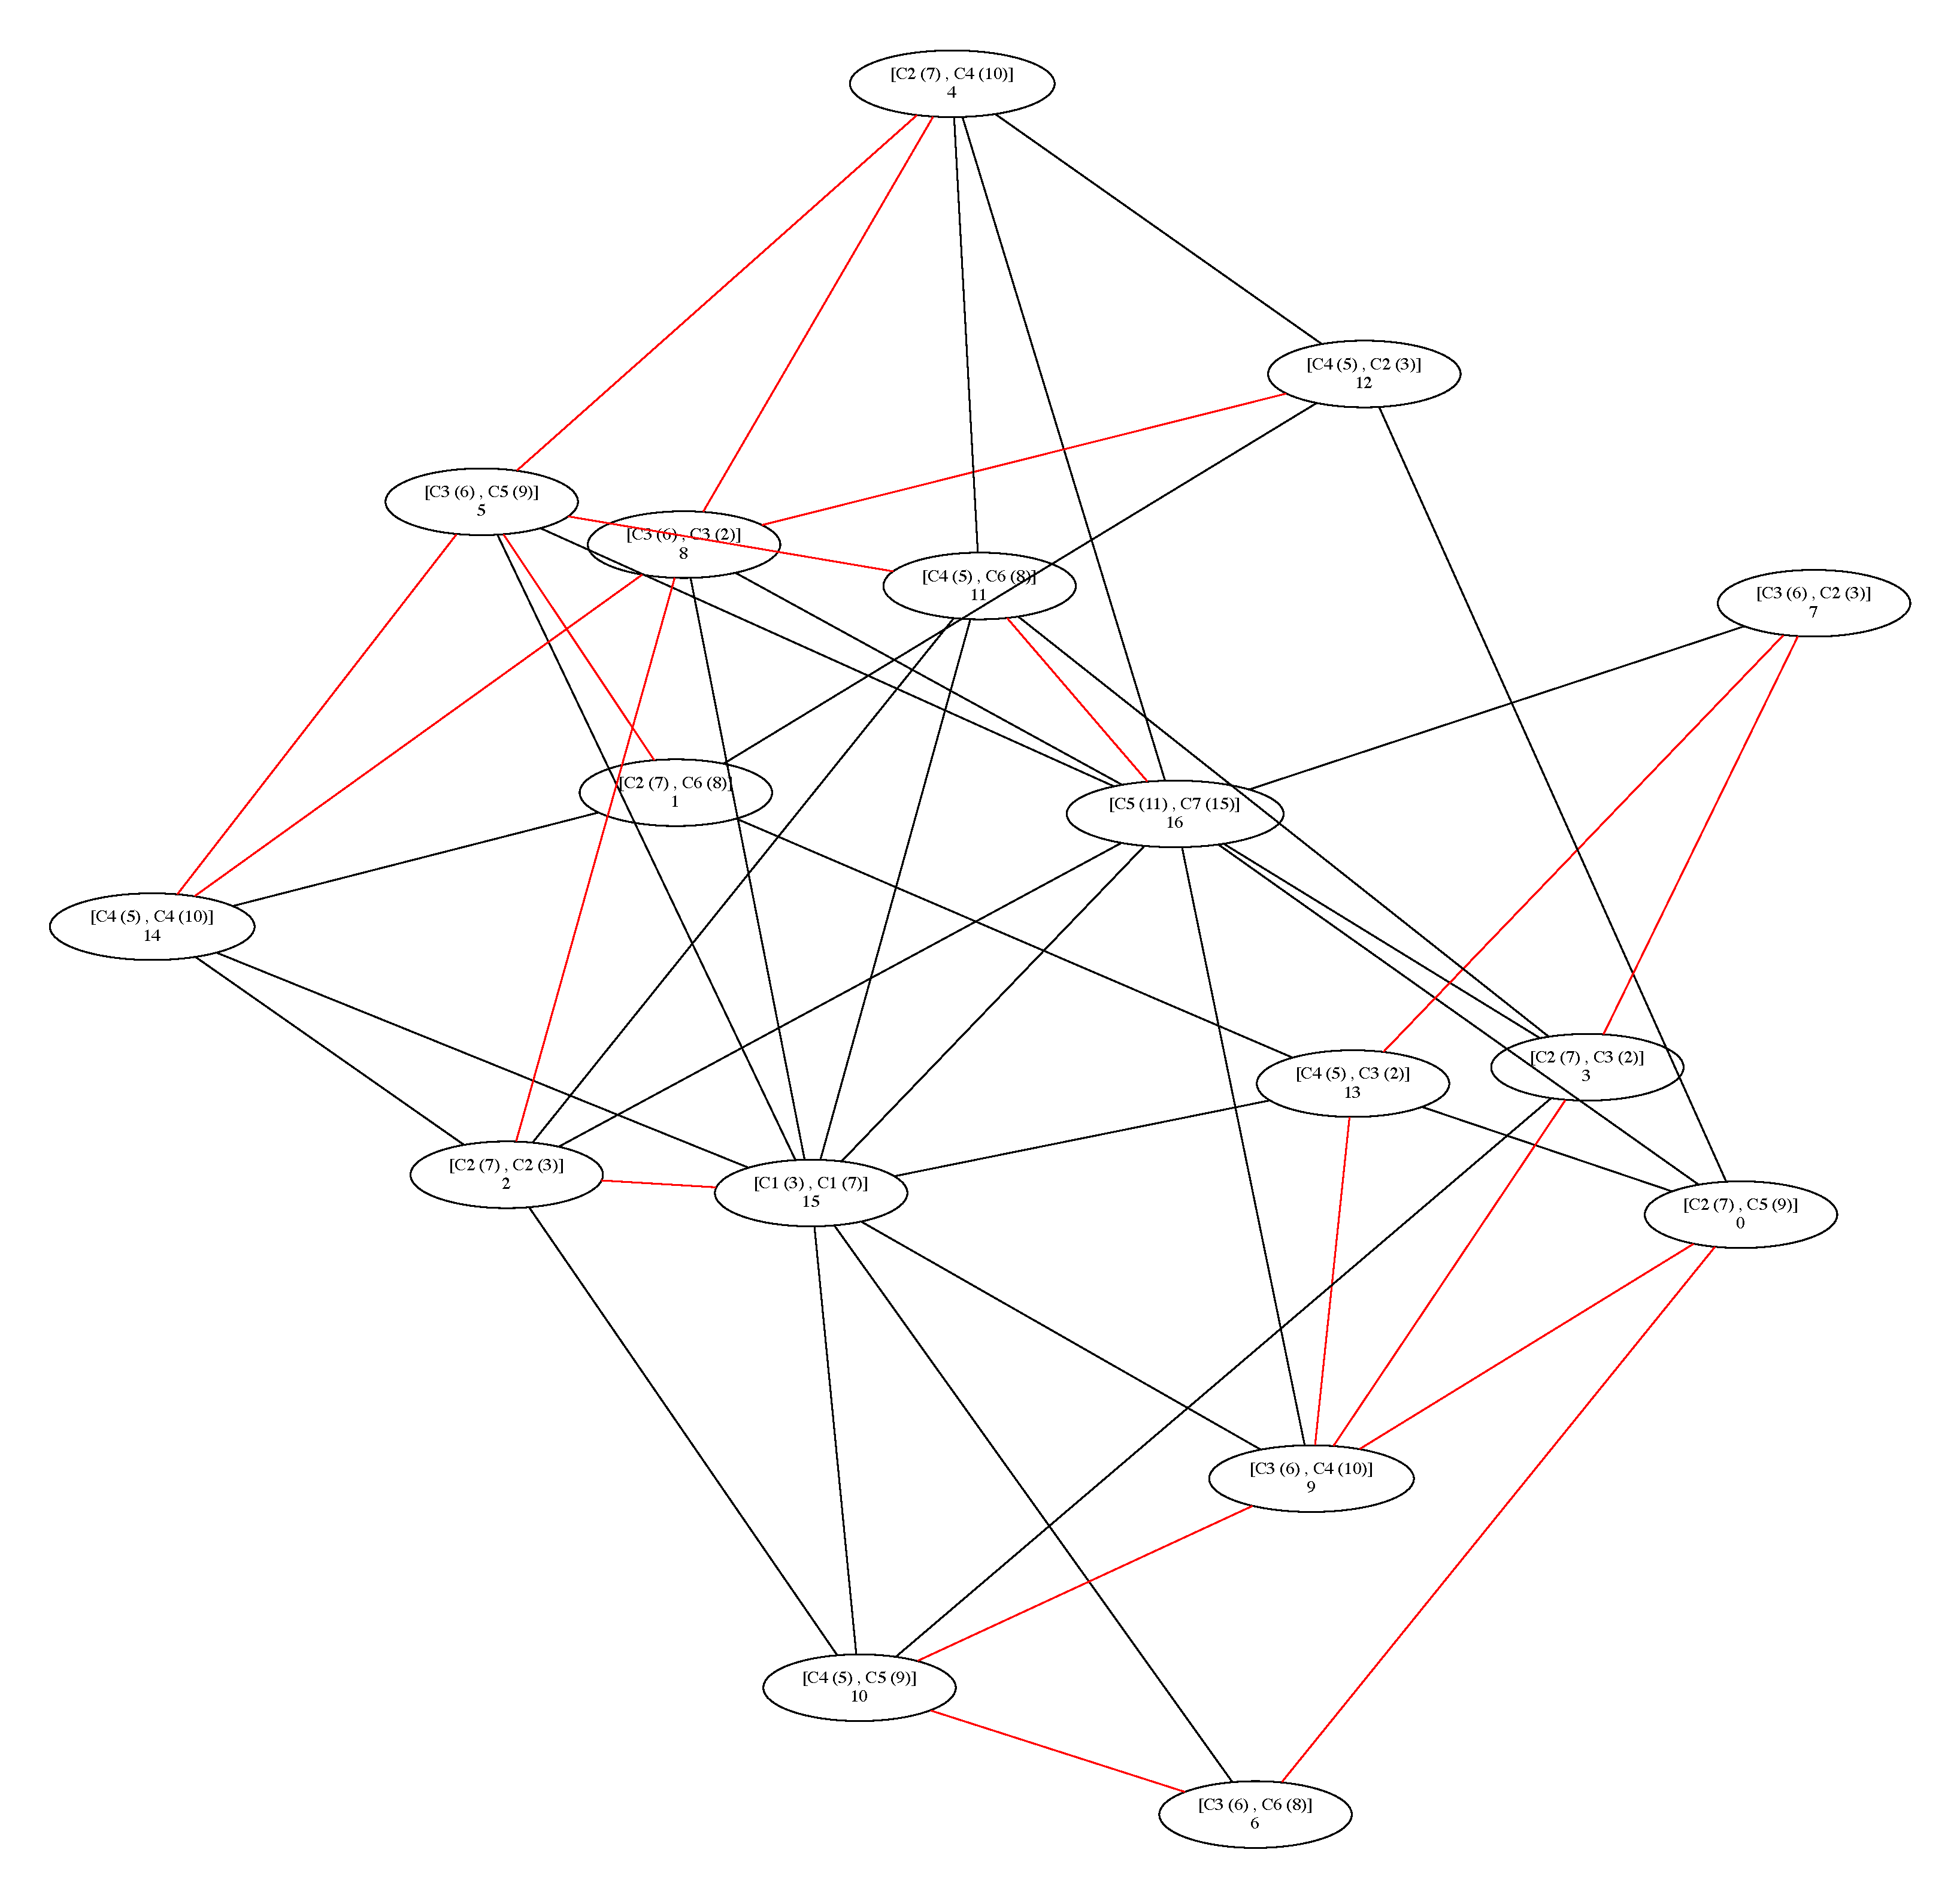
\includegraphics[width=1.1\textwidth]{images/product}
  \caption{The product graph; as an optimization product nodes corresponding to
    degree 1 nodes in the original graphs have been ignored. $c$-edges are
    colored red and $d$-edges are colored black. These are the maximal
    $c$-cliques: $\{10,6\}, \{10,0\}, \{13, 7\},
    \{7, 3\}, \{13, 9, 0\}, \{14, 5, 1\}, \{12, 8, 4\}, \{10, 9, 3\}, \{16, 11,
    5, 4\}$ and $\{15, 14, 8, 2\}$.}
  \label{fig:product}
\end{figure}

We identify maximal $c$-cliques by adapting Bron-Kerbosch' algorithm similarly
to~\cite{Koch:1996fc,Koch:2001wi}.

\begin{algorithm2e}
  \caption{\textsc{BK}$(P,D,R,X,S)$}
  \label{alg:bk-pivot}
  \KwIn{$P$, $D$, $X$ and $S$ are disjoint sets of nodes adjacent to all nodes
    in $R$ whose nodes induce a $c$-clique in $G_{12}$.}
    %All nodes in $P$ are $c$-adjacent to at least one node in $R$. All nodes in
    %$D$ are $d$-adjacent to all nodes in $R$. $R$ defines a maximal $c$-clique.}
  \If{$P \cup X = \emptyset$}{
    Report $R$
  }
  \Else{
    Choose $u \in P \cup X$ maximizing $|P \cap N(u)|$\\
    \ForEach{$v \in P \setminus N(u)$}{
      $P^\prime \leftarrow P \cup (D \cap N_c(v))$\\
      $D^\prime \leftarrow D \setminus N_c(v)$\\
      $X^\prime \leftarrow X \cup (S \cap N_c(v))$\\
      $S^\prime \leftarrow S \setminus N_c(v)$\\
      \textsc{BK}($P^\prime \cap N(v)$, $D^\prime  \cap N(v)$, $R \cup \{v\}$,
      $X^\prime \cap N(v)$, $S^\prime \cap N(v)$)\\
      $P \leftarrow P \setminus \{v\}$\\
      $X \leftarrow X \cup \{v\}$
    }
  }
\end{algorithm2e}

There are five invariants in the algorithm.

\begin{enumerate}
  \item $R$ is a clique.
  \item Each node $v \in P$ is adjacent to all nodes in $R$ and $c$-adjacent to
    at least one node in $R$.
  \item Each node $v \in D$ is $d$-adjacent to all nodes in $R$.
  \item Each node $v \in X$ is adjacent to all nodes in $R$ and $c$-adjacent to
    at least one node in $R$, and all maximal
    $c$-cliques containing $R \cup \{v\}$ have already been reported.
  \item Each node $v \in S$ is $d$-adjacent to all nodes in $R$ and all maximal
    $c$-cliques containing $R \cup \{v\}$ have already been reported.
\end{enumerate}

Invoking \textsc{BK}($P, D, R, X, S$) lists all maximal $c$-cliques in the
subgraph comprised of the nodes in $R$, some of the nodes in $P \cup D$
and none of the nodes in $X \cup S$. So by invoking \textsc{BK}($N_c(v),
N_d(v), \{ v \}, \emptyset, \emptyset$) all maximal $c$-cliques containing $v
\in V_{12}$ will be listed. In fact, the pivot rule we use (line~4,
Algorithm~\ref{alg:bk-pivot}) ensures that every maximal $c$-clique containing
$v$ is listed exactly once~\cite{Tomita:2006kb}. By considering the nodes in a
degeneracy ordering, we can bound the size of $P \cup D$ and arrive at a
worst-case running time of $O(dn3^{d/3})$~\cite{Eppstein:2010uq}---see
Algorithm~\ref{alg:bk-degeneracy}.

\begin{algorithm2e}
  \caption{\textsc{BK}$()$}
  \label{alg:bk-degeneracy}
  Let $v_1, v_2, \ldots, v_n$ be a degeneracy ordering\\
  \For{$i \leftarrow 1$ \KwTo $n$}
  {
    $P \leftarrow N_c(v_i) \cap \{v_{i+1}, \ldots, v_n\}$\\
    $D \leftarrow N_d(v_i) \cap \{v_{i+1}, \ldots, v_n\}$\\
    $X \leftarrow N_c(v_i) \cap \{v_1, \ldots, v_{i-1}\}$\\
    $S \leftarrow N_d(v_i) \cap \{v_1, \ldots, v_{i-1}\}$\\
    \textsc{BK}$(P, D, \{v_i\}, X, S)$
  }
\end{algorithm2e}

\section{Results}

We compiled a repository of fragments based on the lipid data set of the ATB. 
This set contains 151 molecules of sizes varying from 25 up to 285 atoms. 
The computation of all maximal common fragments between the molecule in 
Figure~\ref{fig:16481} and the 151 molecules in the repository takes a 2 seconds. 
For larger molecules, such as the one with molecule id 6401 (145 atoms), 
enumerating all the maximal common fragments takes 2.5 minutes.

\section{Discussion}

Future work includes the following.
\begin{itemize}
  \item How to combine fragments? What about using exact cover, i.e., find a set
    of disjoint maximal common fragments that covers the input molecule?
  \item What is a good repository?
\end{itemize}

\bibliographystyle{abbrv}
\bibliography{fragments}

\end{document}

